\subsection{Broadcast}
\hl{Are application components that can receive 'intents' from other 
components.}

\hl{We can use the broadcast to send information to another app and inside the same app.}

Broadcast receivers can be declared in \textbf{the manifest} or 
\textbf{registered dynamically}. 

They also can have an associated ACTION or cross-application explicit 
intent. 

Are invoked using \texttt{sendBroadcast()}, which can be invoked by
any other component or other application. 

To receive the broadcast message, one must use the \texttt{BroadcastReceiver}. 
It's necessary to override the \texttt{onReceive} class, because this class
doesn't have any user interface. 

Let's create a \texttt{BroadcastReceiver} and declare it in the manifest:

\begin{lstlisting}
...
<application>
...
<receiver android:name=" ... " >
<intent-filter>
<action android:name=" ... " />
</intent-filter>
</receiver>
...
\end{lstlisting}

In the activity, we gonna send the a broadcast message:

\begin{lstlisting}
Intent bi = ... // should match the name of the action in the manifest. 
sendBroadcast(bi);
\end{lstlisting}

An example is: 
\begin{lstlisting}[title=Manifest definition]
<manifest>
    <application>
        ...
        <receiver android:name=".MyReceiver">
            <intent-filter>
                <action android:name="org.feup.intents.test" />
            </intent-filter>
        </receiver>
        ...
    </application>
    ...
</manifest>
\end{lstlisting}

\begin{lstlisting}[title=Broadcast activity]
public class MyActivity extends Activity {
    ...
    private void invokeReceiver() {
        Intent broadcast = new Intent ( "org.feup.intents.test");
        broadcast.putExtra("somename", "Hello");
        sendBroadcast(broadcast);
    }
    ...
}
\end{lstlisting}

\begin{lstlisting}[title=The receiver]
// This class can be instatiated in any component. 
public class MyReceiver extends BroadcastReceiver {
    @Override
    public void onReceive(Context context, Intent intent) {
        String msg = intent.getStringExtra("somename");
        //Do something
    }
}
\end{lstlisting}

\subsection{Services}

\hl{As we have seen before the services are invisible to the user and are not an
asynchronous execution itself.} The \textbf{Service runs in the UI thread}, so it 
can degrade responsiveness and cause ANRs (application not responding), even 
though it does not interact directly with the UI. Still, the \texttt{Service} in 
combination with asynchronous executor is a powerful tool for background task 
execution. 

\subsubsection{Why use a Service for asynchronous execution?}

\begin{itemize}
    \item \textit{Decouple lifecycles of components and threads}: Even after 
    the component that started the thread finishes itself, the thread will continue 
    running. Threads may keep references to Java objects so that they cannot be 
    garbage collected until the thread terminates. 
    \item \textit{Lifecycles of the hosting process}: If the runtime terminates the 
    process, all of its threads are terminated and not restarted by default when the 
    process is restored. A process with no active components is likely yo be eligible 
    for termination, since a task with no components contains low rank. For example, 
    an \texttt{Activity} stores user data to a database in a background thread
    while the user navigates back leaves an empty process if there are no other 
    components running. This increases the risk of process termination, aborting the 
    background thread before it can persist the data. 
\end{itemize}

\hl{Thus, a \texttt{Service} can mitigate both the risk for memory leaks and the risk of 
having tasks terminated prematurely. \textbf{Services has high priority}, but still 
less, than activities.}

\subsubsection{Creation and Execution}

\begin{lstlisting}
    public class EatService extends Service {
        @Override
        public void onCreate() { /* Initialize component */ }
        
        @Override 
        public void onDestroy() {/* Clean up used resources*/} 

        @Override
        public IBinder onBind(Intent intent) { /* Return communication interface */ } 
    }
\end{lstlisting}

The only mandatory method is \texttt{onBind}, which returns the communication 
interface to the client to perform remote call services. 

To \textbf{start} the service, one can call \texttt{startService(Intent)} and to stop 
it's possible to call \texttt{stopService(Intent)} or \texttt{Service.stopSelf()}. 


\begin{figure}[h]
\centering
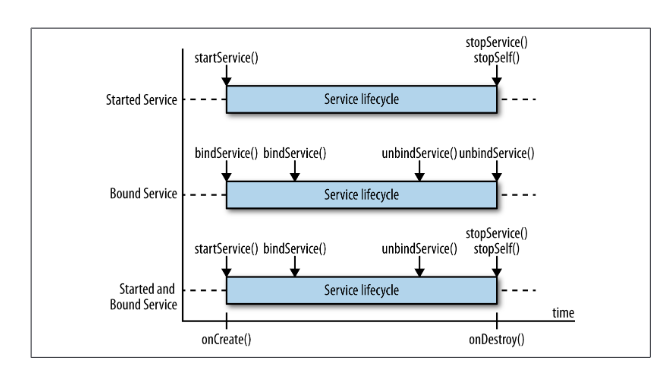
\includegraphics[width=1\linewidth]{figures/06_service_lifecycle.png}
\caption{Service lifecycle}
\label{fig:service_lifecycle}
\end{figure}

\subsubsection{Started service}
Components invoke Context.startService(Intent) to send start requests to a \texttt{Service},
which can be invoked by multiple components and multiple times from every components during 
lifecycle. The first start request creates and starts the \texttt{Service}, whereas consecutive
start requests just pass on the \texttt{Intent} to the started \texttt{Service} so that the
data conveyed in the \texttt{Intent} can be processed. 

Services always have to implement onBind, but started services—which do not support
binding—should provide a trivial implementation that just return null:

\begin{lstlisting}
public class StartedEatService extends Service {
    @Override
    public int onStartCommand(Intent intent, int flags, int startId) { ... }

    @Override
    public IBinder onBind(Intent intent) { return null; }
}
\end{lstlisting}

Started services must implement an \texttt{onStartCommand} method that handles start
requests. The method is invoked each time a start request (\texttt{Context.startService})
from a client component is ready to be processed. 

Start requests are delivered sequentially to onStartCommand and remain pending in 
the runtime until preceding start requests are processed or offloaded from the UI thread.

\begin{tcolorbox}[colback=red!5,colframe=red!75!black, title=Problems of onStartCommand]
onStartCommand is executed on the UI thread, so you should spawn background threads
within the method to execute long-running operations, not only to preserve responsiveness 
but also to enable concurrent execution of multiple start requests.

\end{tcolorbox}

\texttt{onStartCommand} is the key method for implementing started Services and intiating
asynchronous task execution. The arguments are: 

\begin{itemize}
    \item \textit{Intent}: Data to be used for the asynchronous execution; e.g., a URL to a network resource
    that shall be retrieved. 
    \item \textit{Delivery method}: A flag reflecting the history of the start request. 
    This argument may contain other flags in future versions of Android. 
    Possible values are currently 0, START\_FLAG\_REDELIVERY (value of 1), or 
    START\_FLAG\_RETRY (value of 2). 
    \item \textit{StartID}: A unique identifier provided by the runtime for this start request. If the process is
terminated and restarted, onStartCommand is called with the same start ID.
\end{itemize}

The return value of \texttt{onStartCommand} and the second argument (the delivery method flag)
let you control what happens after your \texttt{Service} is terminated. It tells the runtime 
weather to restart the \texttt{Service} and resubmit the \texttt{Intent} argument, in case 
the runtime has to terminate the process for lack of resources and then restart it.

\subsubsection{Options for restarting} 
ike any Android application, your Service may be terminated by the runtime if there 
are too many processes running on the device. In fact, as a background process, your 
Service has a greater chance of being killed than many other processes.

This section covers termination by either the runtime or a client, not a clean termination 
through \texttt{Service.stopSelf}.

The values that the \texttt{onStartCommand} may return are: 
\begin{itemize}
    \item \texttt{START\_STICK}: The \texttt{Service} will be restarted in a new process whether
    or not here are any requests pending. The resources are brought to memory again, but with a 
    \texttt{NULL} intent, because \texttt{onStartCommand} is invoked with a \texttt{null} value for 
    the \texttt{Intent} argument. However, the \texttt{Service} will receive any pending start requests
    that remained undelivered when the previous \texttt{Service} process was terminated. The pending 
    start requests are delivered with the \texttt{START\_FLAG\_RETRY} set in the call's second argument. 

    \item \texttt{START\_NOT\_STICK}: Like \texttt{START\_STICK}, except that the \texttt{Service} will be 
    restarted only if there were pendind start requests when the process was terminated. An \texttt{Intent} will
    always be passed. Then the resources are not brought back to memory until a new \texttt{startService} is
    executed.
    \item \texttt{START\_REDELIVER\_INTENT}: The \texttt{Service} will be restarted and reves both pendind requests
    and requests that were previously started and had no change to finish. The pending requests are 
    delivered with the \texttt{START\_FLAG\_RETRY} set in the second argument, whereas the previously 
    started requests are redelivered with the \texttt{START\_FLAG\_REDELIVERY} set. The resources are 
    brought to memory again with the last process intent. 
\end{itemize}

\subsubsection{Example}

\begin{lstlisting}[title=Service code template]
import android.app.Service;
import android.content.Intent;
import android.os.IBinder;
public class MyService extends Service {
    @Override
    public void onCreate() {
        // TODO: Actions to perform when service is created.
    }
    @Override
    public IBinder onBind(Intent intent) {
        return null; // mandatory but should return null for
        // non remote call services
    }
    @Override
    public int onStartCommand(Intent intent, int flags, int startId) {
        // Usually launch a background thread to do processing.
        return Service.START_NOT_STICKY; // or other value
    }
    @Override
    public void onDestroy() {
        // TODO: Actions to perform when service is destroyed
    }
}
\end{lstlisting}

\begin{lstlisting}[title=Manifest]
    <service android:name=".MyService"/>
\end{lstlisting}

\begin{lstlisting}[title=Calling the service]
// Implicitly start a Service
Intent myIntent = new Intent(MyService.ORDER_PIZZA);
myIntent.putExtra("TOPPING", "Margherita");
startService(myIntent);

// Explicitly start a Service in the same process
startService(new Intent(this, MyService.class));
\end{lstlisting}

\begin{lstlisting}[title=Stoping the service]
// With the same intent
stopService(new Intent(MyService.ORDER_PIZZA));

// Stop a service with the service name (same proc).
ComponentName service = startService(new Intent(this, MyService.class));
...
stopService(new Intent(this, service.getClass()));

// Stop a service explicitly in the same process
Class serviceClass = Class.forName(service.getClassName());
stopService(new Intent(this, serviceClass));
\end{lstlisting}


\subsection{Intent service}
It's a special purpose Service subclass that creates a single worker thread.
The intent received on \texttt{onStartCommand()} is passed to the method that 
the worker thread executes.

The \texttt{IntentService} is suitable for when you want to offload tasks easily 
from the \texttt{UI thread} to a background thread with sequential task processing, 
giving the task a component that is always active in order to raise the process rank.

Successive calls on \texttt{onStartCommand()} are queued. You only have to override and implement
\texttt{onHandleIntent()}. 

\begin{lstlisting}[title=IntentService implementation]
public class MyService extends IntentService {
    public MyService() {
        super("MyService");
    }
    @Override
    protected void onHandleIntent(Intent intent) {
        // Do the work in this single worker thread
        // and return
    }
}
\end{lstlisting}

\subsection{Result Service}
Mechanism to return a result to an \texttt{Activity} (or other component activated by an \texttt{Intent}) from
other component or thread (using a \texttt{Handler()}). 

It is created on the destination with \texttt{onReceiveResult()} overridden.
As this class is \texttt{Parcelable} their objects can be passed in Intent.
The recipient sends results using \texttt{send()}, triggering a call to \texttt{onReceiveResult()}.

\subsubsection{Example}

\begin{lstlisting}[title=Recipient component (an activity)]
//recipient Activity
public class MainActivity extends AppCompatActivity {
    // some variables (Activity state)
    ....
    @Override
    protected void onCreate(Bundle savedInstanceState) {
        ...
        Intent aService = new Intent(this, MyService.class);
        aService.putExtra(MyService.RESULT, new ResultReceiver(new Handler()) {
            @Override
            protected void onReceiveResult(int code, Bundle data) {
                super.OnReceiveResult(code, data);
                .... // if code OK, use data and other Activity state
                ....
            }
        });
    }
}
\end{lstlisting}

\begin{lstlisting}[title=A service sending results]
public class MyService extends Service {
    public final static String RESULT = "RemoteResult";
        ...
    @Override
    public int onStartCommand(Intent i, int flags, int sId) {
        ResultReceiver rec = i.getParcelableExtra(MyService.RESULT);
        ...
        Bundle data = new Bundle();
        data.putString("value", "some data");
        ...
        rec.send(1, data);
        return Service.START_NOT_STICKY;
    }
    ...
}
\end{lstlisting}


\subsection{Remote Call Services (RPC)}

Their functionality is invoked using RPC. Usually, they are standalone in their own processes. 

Remote call services are activated (brought to memory and \texttt{onCreate()} invoked) through
\texttt{bindService()} and can be freed when the last bound client calls \texttt{unbindService()}.

When a service is ready to be called through its interface a callback  \texttt{onServiceConnected()} is 
called on the client.

There is also a \texttt{onServiceDisconnected()} callback on the client that is called when the 
service is not available (motivated by a crash or reclaimed by Android). 

\begin{figure}[h]
\centering
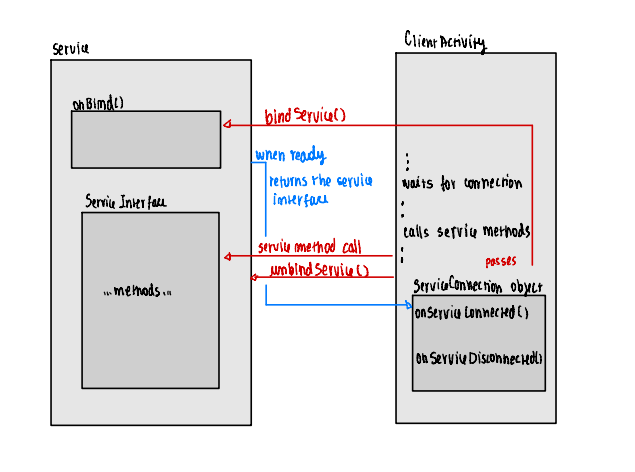
\includegraphics[width=1\linewidth]{figures/06_RPC_flow.png}
\caption{RPC flow}
\label{fig:rpc_flow}
\end{figure}

\subsubsection{Example}

\begin{lstlisting}[title=Service interface is defined in the AIDL file]
// This file is IStockQuoteService.aidl
package com.androidbook.services.stockquoteservice;
    interface IStockQuoteService {
    double getQuote(String ticker);
}
\end{lstlisting}

\begin{lstlisting}[title=Service must implement the interface]
public class StockQuoteService extends Service {
    public class StockQuoteServiceImpl extends IStockQuoteService.Stub {
        @Override
        public double getQuote(String ticker)
            throws RemoteException {
                return 20.0;
            }
        }
    @Override
    public IBinder onBind(Intent intent) {
        return new StockQuoteServiceImpl();
    }
}

\end{lstlisting}

\begin{lstlisting}[title=Client calling the service]
...
bindService(new Intent(IStockQuoteService.class.getName()), serConn, Context.BIND_AUTO_CREATE);
...
private ServiceConnection serConn = new ServiceConnection() {
    @Override
    public void onServiceConnected(ComponentName name, IBinder service) {
        stockService = IStockQuoteService.Stub.asInterface(service);
        callBtn.setEnabled(true);
    }

    @Override
    public void onServiceDisconnected(ComponentName name) {
        callBtn.setEnabled(false);
        stockService = null;
    }
};
...
try {
    double val = stockService.getQuote("ANDROID");
    Toast.makeText(this, "Value from service is " + val, Toast.LENGTH_SHORT) .show();
} catch (RemoteException ee) {
}
\end{lstlisting}

\subsection{Notifications}
Are shown in the status bar. More details listed in the extended status drawer. 
They can produce sound, vibration and light leds. 

They are created using a system service:
\begin{lstlisting}[title=Creating notifications]
String svcName = Context.NOTIFICATION_SERVICE;
NotificationManager notificationManager;
notificationManager = (NotificationManager) getSystemService(svcName);
\end{lstlisting}

Are specified in a Notification object through a Build class:
\begin{lstlisting}[title=Build class]
// A small icon, a title and a text and mandatory (many other features)
// get the Notification object using the build() method
Notification notf = new Notification.Builder(this)
.setContentText(message) // the main text of the notification
.setContentTitle(title) // the first line (title)
.setSmallIcon(R.drawable.nticon) // icon on bar and notification
.setWhen(System.currentTimeMillis()) // for ordering
.setPendingIntent(PendingIntent pi) // Activity to launch on tap
.build(); // returns the notification object
notf.flags |= Notification.FLAG_ONGOING_EVENT; // cannot be cleared
\end{lstlisting}

Sent using the \texttt{notify()} method of the service.

Notifications are customizable. 

\subsection{Alarms}

Calls an application component periodically or after a specified time interval and uses another 
system service: 
\begin{lstlisting}[title=Creating an alarm]
String svcName = Context.ALARM_SERVICE;
AlarmManager alarms;
alarms = (AlarmManager) getSystemService(svcName);
\end{lstlisting}

We can use the methods \texttt{set()}, \texttt{setRepeating()} or \texttt{setInexactRepeating()} to create alarms. 

\begin{lstlisting}
int alarmType = AlarmManager.ELAPSED_REALTIME_WAKEUP;
long timeOrLengthOfWait = 10000;
String ALARM_ACTION = "ALARM_ACTION";
Intent intentToFire = new Intent(ALARM_ACTION);
PendingIntent pendingIntent = PendingIntent.getBroadcast(this, 0, intentToFire, 0);
alarms.set(alarmType, timeOrLengthOfWait, pendingIntent);
\end{lstlisting}








